This chapter introduces this research proposal. It starts with the problem statement, then outlines the motivations, research goals and the organization of this proposal.

\section{Problem Statement}
\label{sec:statement}

\bx{Cloud computing has made a huge impact on modern software industry by offering on-demand computing capacity 
(e.g storage and computing) \cite{2010arxiv1006.0308b}.} Compared with the traditional software industry, where applications run
on individual hardware, on-demand cloud computing provides a cluster of servers for the software industry. For example, 
web service providers such as Google and Neflix deploy their applications on the cloud. These web service providers 
do not need to purchase and maintain hardware resources. 
In addition, they do not need to worry 
about scalability and availability issues when demands of their applications increase. Cloud dynamically increases the capacity of applications and cloud computing services can be accessible 99.99\% of the time~\cite{adhikari:2012uq}.
\qy{Moreover, application users} can enjoy applications without experiencing breakdown and access the applications from anywhere in the world.

\bx{A major issue in cloud computing is the huge energy consumption generated by data centers.}
A typical data center consumes as much energy as 25,000 households \cite{dayarathna:2016ua}. 
This huge energy consumption has become the major expense of cloud providers. It is necessary to find ways to reduce the energy bills. 
The reduction of energy bills would benefit \qy{cloud providers, web service providers and environment.} 
Furthermore, people would pay less to applications on the cloud. 

\bx{Generally, reducing the energy consumption in clouds depends on
improving the resource utilization of live physical machines (PMs) such as servers.} 
Studies show \cite{Barroso:2007jt, Shen:2015hm}, \qy{PMs account for} \qy{the majority} -- more than 40\% -- of energy consumption \qy{in clouds among other components such as cooling systems and network devices}. \qy{Moreover},
these PMs have been not used effectively. \qy{Some studies analyzed }the PMs' average utilization. They found that the average utilization is quite low 
-- from 10\% to 50\% \cite{Hameed:2016cmb}.
Therefore, we can reduce energy by improving the utilization of PMs \qy{and reducing the usage of PMs in clouds}.

\bx{The common way to improve the utilization of PMs in clouds 
is through resource management of PMs \cite{Manvi:2014hm} (see Figure \ref{fig:workflow}).} 
\qy{ A centralized resource management system in clouds}
has two \qy{main} functionalities. \qy{First, the management} system 
allocates resources such as CPUs and memories of PMs \qy{for} cloud users \qy{to run} applications. \qy{Second, the management} system 
handles the workload fluctuations \qy{to reduce the number of potential migrations}. \qy{These two main functionalities deploy and maintain applications in clouds.} 

\bx{The two main functionalities of resource management of PMs in clouds involve four steps.}
First, the management system collects the utilization information of PMs and then 
analyzes the usage of PMs and the resources needed by applications. Next, triggered by resource analysis, the management system determines the 
placement of applications. The placement of applications includes three scenarios: initial placement of applications for new applications; periodic placement of applications for adjusting the running applications periodically; 
and dynamic placement of applications for adjusting applications in a fast manner when abnormal events such as overloading happen. Finally, 
the management system executes the placement decision of applications to PMs. Hence, better management of resources 
in clouds contributes towards a better utilization of PMs and thus a reduction of energy consumption.



\begin{figure}
	\centering
	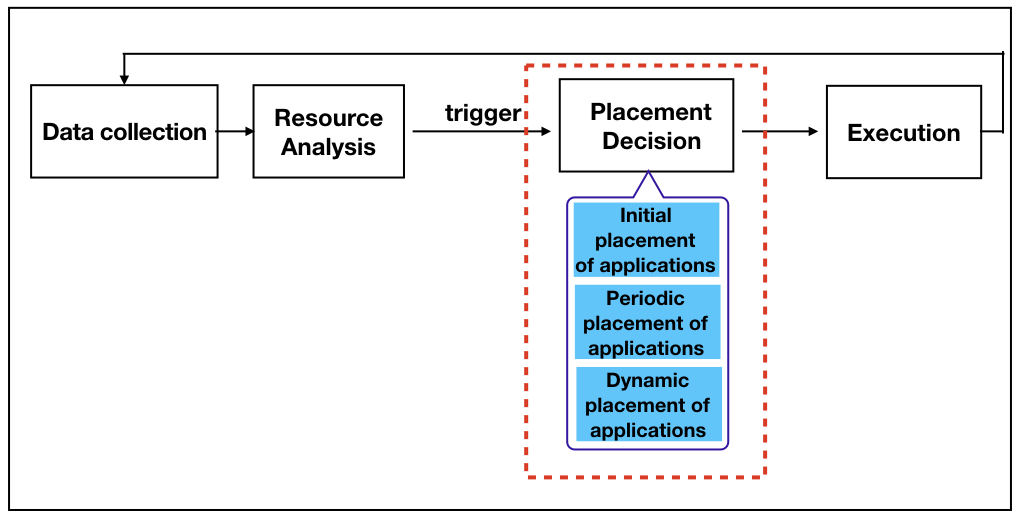
\includegraphics[width=0.8\textwidth]{pics/workflow_management.png}
	\caption{A workflow of resource management \cite{Mishra:2012kx}}
	\label{fig:workflow}
\end{figure}



\bx{The core strategy of resource management is server consolidation \cite{Varasteh:2015fu}.} Two different types of
server consolidation are used in clouds: static and dynamic. Static server consolidation manages resources in an off-line fashion. It is mainly 
used in the initial placement of applications and periodic placement of applications. Dynamic server consolidation manages resources in 
an on-line fashion, which is used in the dynamic placement of applications. Both static and dynamic server consolidation aim to place
applications in fewer PMs. This leads to fewer PMs with higher utilization and lower energy consumption.



\bx{Currently, the resource management in clouds is based on \emph{virtualization} technology\cite{Uhlig:2005do} and the mainstream is virtual machine-based virtualization.}
Such virtualization separates the resources (e.g. CPUs and RAMs) of a PM into several parts called \emph{virtual machines (VMs)}. 
Each VM runs an isolated operating system. This VM-based technology is very different from 
traditional clouds that place each application to a single PM and lead to the low reserved utilization of PMs. 
Compared with traditional clouds, current VM-based clouds significantly improve the utilization of PMs and reduce energy consumption.


\bx{However, in recent years, virtual machine-based virtualization cannot catch up with a new trend in the software industry -- Service Oriented Architecture 
(SOA) \cite{Sprott:2004wt}.} This SOA is widely used in the modern software industry because of its agility and re-usability \cite{Sprott:2004wt}.
SOA separates a centralized application into multiple distributed components called web services. 
As web services only require a small amount of resources (e.g. 15\% of a typical CPU), 
using a VM for a web service causes resource wastage inside a VM. Consequently, the low utilization of PMs decreases
the energy efficiency.


\bx{To support SOA and further reduce energy consumption, a new container-based virtualization~\cite{Felter:2015ki, Soltesz:2007cu} has been proposed.} Containers running on top of 
VMs are called an operating system (OS) level of virtualization~\cite{Soltesz:2007cu}. Similar to VM, 
a container provides performance and resource isolation for a single application. 
Different to VMs, multiple containers can run in the same VM without interfering with each other. 
In addition, containers naturally support \emph{vertical scaling} (change size during runtime)~\cite{Vaquero:2011gb}. 
The vertical scaling provides resilient resources to fluctuate workloads. The container technology provides a new 
architecture for allocating applications and a finer granularity of resource management. Hence, containers have the potential to further
improve the energy efficiency.



\bx{Although the efficient use of containers can improve the utilization of VMs, 
containers bring new challenges and difficulties to server consolidation~\cite{:2017ff}.}
We cannot directly apply current VM-based server consolidation strategies on container-based clouds because 
of the different placement structures of applications. Moreover, to support the increasing size of containers, 
the vertical scaling in clouds requires the VMs to reserve sufficient resources. The interaction between VMs and containers changes 
the server consolidation into a bilevel problem: VMs-to-PMs, and VMs-to-containers. Bilevel problems are NP-hard~\cite{Sinha:2013tn}.  NP-hard means there is no polynomial time algorithm to find the global optimum solution. Therefore, we need to develop better algorithms for the bilevel problem.

\bx{This research aims to improve the energy efficiency in container-based clouds by 
proposing new bilevel energy models and server consolidation algorithms for three placement decision scenarios: }
initial placement of applications, periodic placement of applications, and dynamic placement of applications.


\vspace{5mm}
